\documentclass{article}
\usepackage[legalpaper, textwidth=450pt]{geometry}
\usepackage{amsmath,amssymb}
\DeclareMathOperator{\E}{\mathbb{E}}
\usepackage[utf8]{inputenc}
\usepackage[english]{babel}
\usepackage{biblatex}
\addbibresource{novel.bib}
\usepackage{graphicx}
\usepackage{indentfirst}
\usepackage{physics}
\usepackage{refcheck}
\usepackage{units}
\usepackage{wrapfig}
\usepackage{subcaption}
\usepackage{booktabs}
\usepackage{multirow}
\usepackage{graphicx}
\setkeys{Gin}{width=.6\textwidth}
\graphicspath{ {./images/} }

\newtheorem{proposition}{Proposition}

\newenvironment{proof}
 {\begin{trivlist} \item[] {\bf Proof.\ }}{\hfill$\Box$ \end{trivlist}}

\title{Newsvendor Problems: A New Integrated Approach\\ to Forecasting and Optimisation}

\author{Congzheng Liu\thanks{Department of Management Science,
Lancaster University, Lancaster LA1 4YX, UK.
Email: {\tt \{c.liu19,a.n.letchford,i.svetunkov\}@lancaster.ac.uk}}
\and Adam N.\ Letchford$^*$ \and Ivan Svetunkov$^*$} % end author list

\date{Draft, 13th June 2020}

\begin{document}

\maketitle

\begin{abstract}
Newsvendor problems form a classical and important family of stochastic optimisation problems. The standard solution approach decomposes the problem into two steps: estimation of the demand distribution, then determination of the optimal production quantity (or quantities) for the given distribution. We propose a new, integrated solution approach, which estimates the optimal production quantity directly from the data. Our approach can be used even when the demand distribution is not stationary. Some encouraging computational results are given. 
\\*[2mm]
{\bf Keywords:} newsvendor problems, forecasting, data-driven optimisation, sales and operations planning
\end{abstract}


%%%%%%%%%%%%%%%%%%%%%%%%%%%%%%
\section{Introduction}

Inventory control is a classical and important topic in Operations Research and Operations Management (see, e.g., the books \cite{Po02,SPP98,Zi00}). In this paper, we focus on \emph{Newsvendor Problem} (NVP), which referrs to a \emph{single-period} \emph{stochastic} inventory control problem.

In early works on NVP \cite{AHM51,MK51}, it is assumed that the demand in each time period comes from a known probability distribution. Of course, in practice, this is not the case --- a fact already noted in 1958 by Scarf \cite{Sc58}. Assuming that historical demand data is available, one can attempt to address this difficulty by decomposing the problem into an estimation / forecasting phase and an optimisation phase.
In the first phase, one makes some assumption (e.g., normality) regarding the underlying data generating process, and uses the past data to estimate the parameters of the process.
In the second phase, one determines the order quantity (or quantities) based on the estimated parameter values.

Throughout this paper, we will call this two-phase approach the \emph{disjoint} approach. An advantage of the disjoint approach is that forecasting and optimisation experts can operate independently within an organisation. This makes things easier to manage. On the other hand, as noticed by several authors \cite{BT06,BM12,Ka94,KT96,KTB20}, there are two disadvantages:
\begin{itemize}
\item The two phases use different objective functions. Indeed, in the first phase, the objective is to minimise a function of the forecasting errors, such as the root mean square error or mean absolute error. In the second phase, however, the goal is usually to maximise expected profit.
\item If the forecasting model is misspecified, and/or there is substantial noise in the data, the effect on the optimisation phase is very hard to predict. In particular, upside and downside errors may have very different effects on expected profit.
\end{itemize}

An alternative to the disjoint approach is to use a single, \textit{integrated} approach, in which the order quantities are determined directly from the data. A simple example of an integrated approach is \emph{quantile regression} \cite{Br16,Hu19}. A nice feature of quantile regression is that it makes no assumptions about the demand distribution. Unfortunately, it can only be applied to relatively simple NVPs, for which one can express the optimal order quantities in terms of quantiles of demand.

In this paper, we introduce a new integrated approach. It is very flexible, and can be applied to a wide variety of NVPs, with complex profit functions. Roughly speaking, it involves forecasting the optimal order quantities instead of the demand. Moreover, instead of determining parameter values that minimise some function of the forecasting errors, our approach attempts to maximise the expected profit directly.

After explaining our approach formally, we show that it reduces to quantile regression in the case of the simplest NVP (with only one product, stationary demand, and linear profit functions).  We then perform extensive computational experiments, on several different NVPs. The results show that our method performs well, in comparison with the disjoint approach, according to several different measures of quality.

The rest of the paper is organized as follows. Section \ref{se:lit} provides a brief review of the relevant literature. Section \ref{se:new} presents the new method and shows that it is a generalisation of quantile regression. In Section \ref{se:results}, we present and discuss the computational results. Finally, Section \ref{se:end} gives some insights, remarks and suggestions.

%%%%%%%%%%%%%%%%%%%%%%%%%%%%%%
\section{Literature Review} \label{se:lit}

Since the literature on NVPs is vast, we mention here only works of direct relevance. The reader looking for more information is directed to the books \cite{Ch12,Po02,SPP98,Zi00}.

\subsection{The classical newsvendor problem} %\label{sub:lit1}

In the simplest NVP, found in textbooks \cite{Ch12}, a company purchases goods at the beginning of a time period at a cost of $v$ per unit, and aims to sell them by the end of the period at a price $p$ per unit. The demand during the period is a random variable $Y$ with known probability density function $f$ and cumulative distribution function $F$. At the end of the period, any surplus goods will lead to a \emph{holding cost} of $c_h$ per unit. On the other hand, shortage of goods during the period will lead to a \emph{shortage cost} of $c_s$ per unit. The goal is to determine an \emph{order quantity} $Q$, prior to the period, that maximises the expected profit.

For a given $Q$ and a given realisation $y$ of $Y$, the profit over the period is:
\[
    \pi(Q,y)=
    \begin{cases}
        py-vQ-c_h(Q-y),& \text{if } Q\geq y\\
        pQ-vQ-c_s(y-Q),& \text{if } Q< y.
    \end{cases}
\]
The expected value of $\pi(Q,y)$ is:
\[
    \Pi(Q) = \int_{0}^{Q} \big[ py-vQ-c_h(Q-y) \big] f(y)dy + \int_{Q}^{\infty} \big[ pQ-vQ-c_s(y-Q) \big] f(y)dy.
\]

It is common to call $c_u= p-v+c_s$ the ‘underage’ cost and $c_o = v+c_h$ the ‘overage’ cost. Some calculus then shows that the order quantity that maximises $\Pi(Q)$ is:
\[
    Q^* = F^{-1}\left( \frac{c_u}{c_o+c_u} \right),
\]
where $F^{-1}$ is the inverse function of $F$. Thus, $Q^*$ is the $\tau$\textsuperscript{th} quantile of $f$, with $\tau=\nicefrac{c_u}{(c_o+c_u)}$.

\subsection{More complex newsvendor problems} %\label{sub:lit2}

Since the NVP was introduced in the 1950s \cite{AHM51,MK51}, researchers have considered several extensions of the problem, including variants with multiple product types \cite{HW63,LL96,MS00}, quantity discounts \cite{Kh95}, different risk measures \cite{EGS95}, product substitution \cite{BAA99}, nonlinear cost functions \cite{HOS12}, non-stationary demand \cite{KWH15}, and price setting \cite{KC62,Mi59,PD99}.

For the purpose of what follows, we now explain one variant, the `Nonlinear Newsvendor Problem' (NNVP), in detail (see also \cite{BT06,HOS12,HN16,KC62,Kh95,KK18,Mi59,PSC15,PD99}). In the NNVP, the profit function takes the form:
\[
    \pi(Q,y)=
    \begin{cases}
        P(Q,y)-V(Q)-C_h(Q,y),& \text{for } Q \geq y\\
        P(Q,y)-V(Q)-C_s(Q,y),& \text{for } Q< y,
    \end{cases}
\]
where $V$, $P$, $C_h$ and $C_s$ are now \emph{functions} rather than constants.

If $\pi(Q,y)$ has a particularly simple form (e.g., if it is piecewise-linear), then it may be possible to  use calculus to express the optimal order quantity as a quantile. In general, however, a closed-form expression as a quantile is unlikely to exist.

We now review one particular NNVP, taken from \cite{KK18,PD99,RK02}, that we are going to use in our numerical experiments. The purchase cost $v$ and selling price $p$ are constants, but $C_h$ and $C_s$ are functions. Overstock items incur a fixed unit penalty $\alpha > 0$, but they can be sold in a salvage market with fixed unit sales price $\beta$, with $0<\beta<v$. The demand in the salvage market is itself a random variable, with known distribution, which we denote by $u$. That is, we have:
\[
    C_h(Q,y) \, = \, \alpha[Q-y]^{+} - \beta \E \Big[ \min \big\{ [Q-y]^{+},u \big\} \Big].
\]
Moreover, the shortage penalty is proportional to the shortage quantity. That is:
\[
C_s(Q,y) =  \zeta \, \big( [y-Q]^{+} \big)^2
\]
for some constant $\zeta > 0$.

\subsection{Quantile regression} %\label{sub:lit3}

Returning to the classical NVP, we now consider the (more realistic) case in which the demand distribution is unknown, but we have historical demands $y_1,y_2,\dots,y_s$.
For this case, \emph{quantile regression}
has proven to perform rather well. The basic idea is as follows \cite{BT06,Br16,CS19,HNS15,Hu19}:
\begin{enumerate}
\item Compute the value of $\tau$ that maximises expected profit;
\item Use quantile regression to compute an estimate of the $\tau$\textsuperscript{th} quantile of the demand in the next time period, which we denote by $\hat{y}_{s+1}^{(\tau)}$;
\item Set the order quantity $\hat{Q}_{s+1}$ to $\hat{y}_{s+1}^{(\tau)}$.
\end{enumerate}

Unfortunately, quantile regression is efficient only on large samples \cite{Hu19,RV19}. Another drawback is that the performance of this approach depends crucially on the underlying target service level. In the experiments of Huber \cite{Hu19} and Rudin \cite{RV19}, the benefit of using the quantile regression method is limited to target service levels smaller than 0.8.

\subsection{Other integrated approaches} %\label{sub:lit4}

There exist other integrated methods. One approach is to use machine learning techniques, such as neural networks, to estimate the optimal order quantity from historical data. The application of machine learning to NVPs can be seen in \cite{CS19,OST20,RV19}. Another integrated approach is based on so-called \emph{one-shot decision theory} \cite{Guo11,GM14,Ma19}. A numerical example was shown in \cite{Guo11}, and extensions can be found in \cite{Ma19}. For the sake of brevity, we do not describe these alternative integrated methods in detail.

%%%%%%%%%%%%%%%%%%%%%%%%%%%%%
\section{The Proposed Estimator for NVPs} \label{se:new}

We have seen that, while quantile regression can be an attractive integrated approach, it has some drawbacks. In particular, for most non-trivial NVPs, it is very hard to express the optimal order quantity as a demand quantile \emph{a priori}. In order to overcome this limitation, we propose an alternative integrated method, based on a regression model with a specialised loss function.

For each historical period $t\in [1,s]$, we assume that the observed demand $y_t$ was a realisation of a random variable $Y_t$. Then, in principle, there exists an order quantity, say $Q_t^*$, that maximises the expected profit given $Y_t$ and $\Pi$. Thus, if we had set $Q_t$ to $Q_t^*$ prior to observing the true demand $y_t$, we would have maximised our expected profit in period $t$. Putting it another way, if we could somehow uncover the hidden structure of the time series $\big\{ Q_1^*,\dots,Q_s^* \big\}$, we would be able to estimate $Q_{s+1}^*$ directly.

Of course, in practice, the distributions $Y_t$ are unknown, and the values $Q_t^*$ are not observable. So we approximate the $Q_t^*$ values using a linear regression model. For each $t$, the regression model yields an estimate of $Q^*_t$, which we denote by $\hat{Q}_t$. The estimate $\hat{Q}_{s+1}$ can then be used as the order quantity in the next time period.

The crucial feature of our approach is that, instead of using the standard least-squares loss function to estimates the regression parameters, we choose the parameters that maximise the expected profit function $\sum_{t=1}^s{\pi \big( \hat{Q}_t,y_t \big)}$. In more detail, we wish to compute the vector
\[
    \hat{\boldsymbol{\beta}}=\text{argmax}_{\boldsymbol{\beta}\in \mathbb{R}^{p+1}}\displaystyle\sum_{t=1}^s{\pi(\hat{Q}_t,y_t)},
\]
based on the assumption of a linear relationship of the form
\[
    \mathbf{\hat{Q}}=\mathbf{X}\boldsymbol{\beta},
\]
where
\[
    \mathbf{\hat{Q}}=
    \begin{pmatrix}
        \hat{Q}_1\\
        \hat{Q}_2\\
        \vdots\\
        \hat{Q}_s
    \end{pmatrix}, \quad
    \mathbf{X}=
    \begin{pmatrix}
        \mathbf{x}_1^{\mathsf{T}}\\
        \mathbf{x}_2^{\mathsf{T}}\\
        \vdots\\
        \mathbf{x}_s^{\mathsf{T}}
    \end{pmatrix}=
    \begin{pmatrix}
        1&x_{11}&\cdots &x_{1p}\\
        1&x_{21}&\cdots &x_{2p}\\
        \vdots &\vdots &\ddots &\vdots \\
        1&x_{s1}&\cdots &x_{sp}
    \end{pmatrix}, \quad
    \boldsymbol{\beta}=
    \begin{pmatrix}
        \beta_0\\
        \beta_1\\
        \beta_2\\
        \vdots\\
        \beta_{p}
    \end{pmatrix}.
\]
Here, $\mathbf{x}_t^{\mathsf{T}}$ is the $t$th row of matrix $\mathbf{X}$,
and $p$ is the number of explanatory variables.

After estimating the model, we can set our next order quantity to $\hat{Q}_{s+1}$. We remark that, while we focus on the linear regression model in this paper, dynamic models, such as ARIMA or ETS \cite{HKO08}, could be used instead just as efficiently. 

It turns out that, in the case of the classical NVP, the proposed estimator has the following statistical properties:
\begin{proposition}[Scale and shift invariance]
For any $a>0$, $\gamma\in \mathbb{R}^{p+1}$ and $\tau\in[0,1]$, we have
\[
    \hat{\boldsymbol{\beta}}(a\mathbf{y},\mathbf{X})=a\hat{\boldsymbol{\beta}}(\mathbf{y},\mathbf{X}).
\]
\[
    \hat{\boldsymbol{\beta}}(\mathbf{y}+\mathbf{X}\gamma,\mathbf{X})=
    \hat{\boldsymbol{\beta}}(\mathbf{y},\mathbf{X})+\gamma.
\]
\end{proposition}
\begin{proof}
See Appendix \ref{app:A}.
\end{proof}

\begin{proposition}[Invariance under reparameterization]
Given any $(p+1)\times (p+1)$ non-singular matrix $A$, we have
\[
        \hat{\boldsymbol{\beta}}(\mathbf{y},\mathbf{X}A)=A^{-1}\hat{\boldsymbol{\beta}}(\mathbf{y},\mathbf{X}).
\]
\end{proposition}
\begin{proof}
See Appendix \ref{app:B}.
\end{proof}

Another interesting feature of our method is that it reduces to quantile regression in the case of the classical NVP. For a proof, see Appendix \ref{app:C}. Therefore, again in the classical case, our estimator
inherits the desirable properties of quantile regression, such as
consistency \cite{Koe05}, efficiency \cite{KM99} and asymptotic
normality \cite{KHM05}.

%%%%%%%%%%%%%%%%%%%%%%%%%%%%%%
\section{Computational Experiments} \label{se:results}

\subsection{Simulation design}

In this section, we conduct the simulation experiment in order to demonstrate the performance of the proposed method. The data are simulated from ARIMA $(1,0,0)(1,0,0)_4$ with $\theta=0.3,\Theta=0.5$ and constant level $=500$. The simulation will be performed base on 20,000 iterations. We consider the simplest scenario in the beginning, where the underlying profit function is linear, the error term of the demand follows normal distribution $\mathcal{N}(0,200^2)$, and we know the model of the data generating process. Specifically, we consider three profit functions \footnote{
The parameters of three profit functions are:
\begin{enumerate}
    \item $p=20$, $v=8$, $c_h=-3$, $c_s=-7$
    \item $p=20$, $v=8$, $c_h=3$, $c_s=7$
    \item $p=20$, $v=10$, $c_h=-3$, $c_s=-7$
\end{enumerate}
} whose optimal order solutions denote three different target service levels (0.5, 0.63 and 0.3).

To further explore the method, we consider five data sizes (40,120,480,1200,4800) in order to see how the proposed method performs when the learning period varies.

In the experiment, we use seasonal dummies and lag term 1 and 4 as explanatory variables for the proposed method. Besides, two benchmark methods are selected to compare performance with:
\begin{itemize}
    \item Disjoint method that use ARIMA $(1,0,0)(1,0,0)_4$ to forecast in the first phase and determine the optimal quantile from the profit function in the second phase,
    \item Integrated method that use Quantile Regression with seasonal dummies and lag term 1 and 4 as explanatory variables.
\end{itemize}
Moreover, we use the results of the exact model and parameters from data generating process to be our upper bound. We build the proposed method and benchmark methods based on the given data set, and compare their performance on the $1$-step ahead forecast. The comparison of performance includes:
\begin{enumerate}
    \item Percentage Profit Loss ($PPL=\frac{\pi(y_{s+1},y_{s+1})-\pi(\hat{Q}_{s+1},y_{s+1})}{\pi(y_{s+1},y_{s+1})}$),
    \item Service Level ($SL=\mathbb {I}_{(\hat{Q}_{s+1}>y_{s+1})}$),
    \item Fill Rate ($FR=\frac{\min\{\hat{Q}_{s+1},y_{s+1}\}}{y_{s+1}}$).
\end{enumerate}

The results are presented in tables and figures. In Figure \ref{fig:ppl0.3}, average percentage profit loss are calculated based on iterations. Particularly, this figure represents the average performance of methods regarding to percentage profit loss in the situation where the target service level $=0.3$. DGP denotes the exact ARIMA model and parameters from data generating process, DJ denotes the disjoint method, QR denotes the quantile regression method, and CF denotes our proposed method. We can see both the proposed method and the benchmark methods converge to the upper bound when data size grows. Besides, the performance of our proposed method and quantile regression is very similar. This is exactly what we expected base on the transformation property we proved in Section \ref{se:new}. However, when the data size is small, the disjoint method performed slightly better than the quantile regression method and the proposed method. 

\begin{figure}[ht]
\centering
\caption{Percentage profit loss vs. data size at 0.3 target service level}
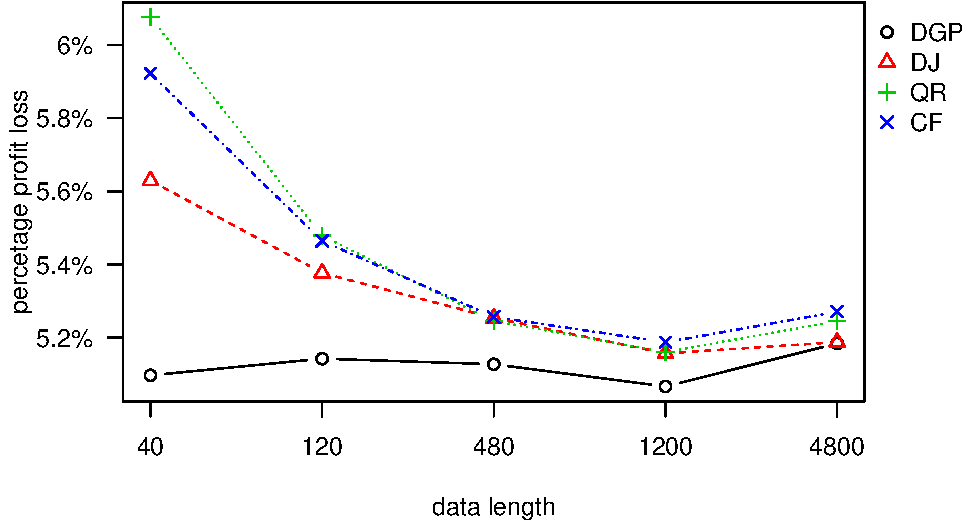
\includegraphics{ppl0.3-1.pdf}
\label{fig:ppl0.3}
\end{figure}

Figure \ref{fig:sl0.3} represent the proportion of iterations that the demand is satisfied (e.g. 0.32 means the demand are satisfied in 6,400 of the 20,000 iterations). We can see that both the three methods and the DGP converge to the target service level 0.3 when data length grows. Yet, the disjoint method approaches the target service level from lower side while the proposed method and the quantile regression approach it from upper side. This phenomenon could be explained by the difference in mechanisms of the disjoint method and integrated method. The disjoint method forecasts the mean and variance of the demand distribution in the first phase. When the data size is small, the forecasted variance will be much bigger than the true variance. The variance, however, plays important role in determining quantile in the second phase. Therefore, bigger variance makes the solution of the optimal quantity 'far away' from 0.5, which leads to lower service level than target. On the other hand, the integrated method approaches the true optimal quantity by applying the optimisation algorithm directly on total profit. Therefore, even if there are two quantity value that have equal distance from the optimal quantity, the algorithm will always favor the one with better profit. In this particular profit function, the algorithm will always favor the quantity with higher service level.

\begin{figure}[ht]
\centering
\caption{Service level vs. data size at 0.3 target service level}
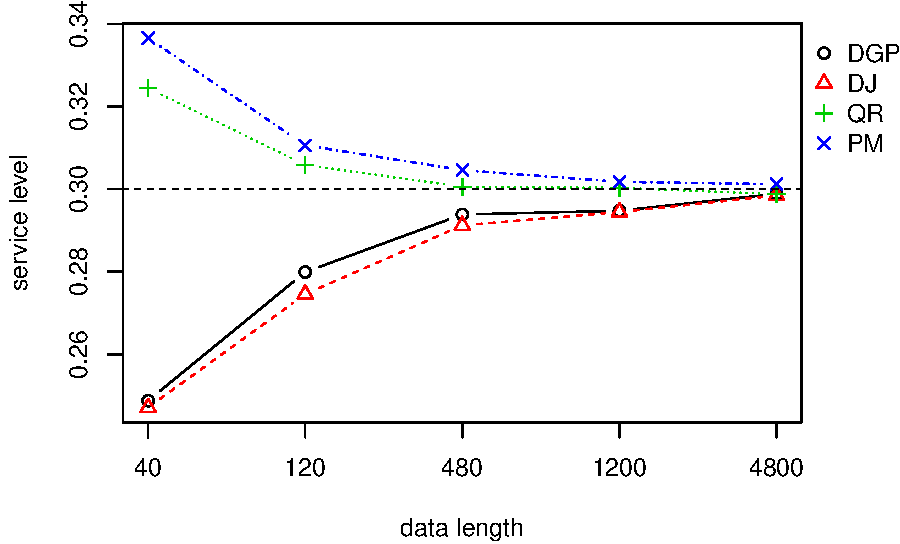
\includegraphics{sl-3.pdf}
\label{fig:sl0.3}
\end{figure}

By fixing the target service level, we can compare the performance of methods in different data size in Table \ref{tab:size_effect0.3}. The value in columns of percentage profit loss and service level are in line with the results in Figure \ref{fig:ppl0.3} and Figure \ref{fig:sl0.3}. The columns of fill rate, on the other hand, provide us more information about demand fulfilment. The service level represents the proportion of iterations that the demand is satisfied, while the fill rate not only provides whether the demand is satisfied or not, but also provides in what percentage the demand is filled. In the case demand is not satisfied, it is well expected that the gap of inventory is as small as possible. In Table \ref{tab:size_effect0.3}, we can see that the proposed method maintains a very high fill rate in all data size. 

\begin{table}[ht]
\caption{Size effect at 0.3 target service level}
\label{tab:size_effect0.3}
\centering \resizebox{\linewidth}{!}{
\begin{tabular}[t]{ccccccccccccc}
\toprule
\multicolumn{1}{c}{\textbf{ }} & \multicolumn{4}{c}{\textbf{Percentage profit loss}} & \multicolumn{4}{c}{\textbf{Service level}} & \multicolumn{4}{c}{\textbf{Fill rate}} \\
\cmidrule(l{3pt}r{3pt}){2-5} \cmidrule(l{3pt}r{3pt}){6-9} \cmidrule(l{3pt}r{3pt}){10-13}
Data size & DGP & disjoint & quantile & proposed & DGP & disjoint & quantile & proposed & DGP & disjoint & quantile & proposed\\
\midrule
40 & 5.1\% & 5.6\% & 6.1\% & 5.9\% & 0.25 & 0.24 & 0.33 & 0.33 & 89.5\% & 88.0\% & 90.0\% & 90.8\%\\
120 & 5.1\% & 5.4\% & 5.5\% & 5.5\% & 0.28 & 0.28 & 0.31 & 0.31 & 90.6\% & 89.7\% & 90.7\% & 91.0\%\\
480 & 5.1\% & 5.3\% & 5.2\% & 5.3\% & 0.29 & 0.29 & 0.30 & 0.30 & 90.9\% & 90.5\% & 90.9\% & 91.0\%\\
1200 & 5.1\% & 5.2\% & 5.2\% & 5.2\% & 0.30 & 0.29 & 0.30 & 0.30 & 91.1\% & 90.7\% & 91.0\% & 91.1\%\\
4800 & 5.2\% & 5.2\% & 5.2\% & 5.3\% & 0.30 & 0.30 & 0.30 & 0.30 & 91.0\% & 90.9\% & 90.9\% & 91.0\%\\
\bottomrule
\end{tabular}} 
\end{table}

On the other hand, we can also compare the methods' performance regarding to different target service levels while fix the data size as in Table \ref{tab:level_effect40} and Table \ref{tab:level_effect4800}, which represent the case data is insufficient and the case data is abundant, respectively. We can see that in both tables, the percentage profit loss of all methods is particular high at 0.63 target service level. It is due to the opportunity cost is different in each profit function. In the function at 0.63 target service level, the 'underage' cost is 19 and the 'overage' cost is 11. However, in the function at 0.3 target service level, those costs are 3 and 7. This high opportunity cost leads to severe overstock/understock punishment, and affects percentage profit loss. As we can see in Table \ref{tab:level_effect4800}, all methods perform similarly when data is sufficient. This result is in line with Figure \ref{fig:ppl0.3} and Figure \ref{fig:sl0.3} where target service level is 0.3. In Table \ref{tab:level_effect40}, where the data size is small, we can see that both the proposed method and benchmarks methods generate acceptable percentage profit loss compared with DGP. Yet, the service level of disjoint method is very poor in all cases. This phenomenon is in line with the findings from Figure \ref{fig:sl0.3}.

\begin{table}[ht]
\caption{Target service level effect on percentage profit loss and service level at 40 data size}
\label{tab:level_effect40}
\centering
\resizebox{\linewidth}{!}{
\begin{tabular}[t]{ccccccccc}
\toprule
\multicolumn{1}{c}{\textbf{ }} & \multicolumn{4}{c}{\textbf{Percentage profit loss}} & \multicolumn{4}{c}{\textbf{Service level}} \\
\cmidrule(l{3pt}r{3pt}){2-5} \cmidrule(l{3pt}r{3pt}){6-9}
Target service level & DGP & disjoint & quantile & proposed & DGP & disjoint & quantile & proposed\\
\midrule
0.5 & 2.4\% & 2.7\% & 2.7\% & 2.7\% & 0.50 & 0.39 & 0.50 & 0.50\\
0.63 & 7.1\% & 7.6\% & 7.8\% & 7.5\% & 0.74 & 0.56 & 0.59 & 0.60\\
0.3 & 2.7\% & 3.0\% & 2.9\% & 2.8\% & 0.15 & 0.18 & 0.33 & 0.34\\
\bottomrule
\end{tabular}}
\end{table}

\begin{table}[ht]
\caption{Target service level effect on percentage profit loss and service level at 4800 data size}
\label{tab:level_effect4800}
\centering
\resizebox{\linewidth}{!}{
\begin{tabular}[t]{ccccccccc}
\toprule
\multicolumn{1}{c}{\textbf{ }} & \multicolumn{4}{c}{\textbf{Percentage profit loss}} & \multicolumn{4}{c}{\textbf{Service level}} \\
\cmidrule(l{3pt}r{3pt}){2-5} \cmidrule(l{3pt}r{3pt}){6-9}
Target service level & DGP & disjoint & quantile & proposed & DGP & disjoint & quantile & proposed\\
\midrule
0.5 & 2.4\% & 2.4\% & 2.4\% & 2.4\% & 0.51 & 0.50 & 0.51 & 0.51\\
0.63 & 6.7\% & 6.7\% & 6.8\% & 6.8\% & 0.64 & 0.64 & 0.64 & 0.64\\
0.3 & 2.5\% & 2.5\% & 2.5\% & 2.5\% & 0.30 & 0.30 & 0.30 & 0.30\\
\bottomrule
\end{tabular}}
\end{table}

\subsection{Misleading model information}
In this subsection, we consider the performance of our proposed method, compared with the disjoint method, in the scenario where we possess misleading model information. The data is still generated from ARIMA $(1,0,0)(1,0,0)_4$ model, while two misleading model are considered, AR$(1)$ and ARIMA $(2,0,0)(1,0,0)_4$. To fairly compare performance with those two disjoint model, we use lag term 1 as explanatory variable for the proposed method in first model and lag term 1, 2, 4 as explanatory variable for the proposed method in second model. As in the previous scenario, the error term of the demand follows normal distribution. In this experiment, we use a linear profit function where $p=20$, $v=10$, $c_h=-3$, $c_s=-7$, and fix the target service level to be 0.3. The percentage profit loss of different data size for the misleading model can be seen in Figure \ref{fig:mis}. It is clear that both the disjoint method and our proposed integrated method generate high percentage profit loss in all data size when the misleading model is AR$(1)$. Obviously, short of explanatory variables makes the forecasting less accurate. In the case where misleading model is ARIMA $(2,0,0)(1,0,0)_4$, our forecasting methods can capture the structure when data is sufficient. However, we can see that when data size is small, the misleading information still has some influence on the performance. Moreover, disjoint method performs slightly better than the proposed method at small data size. Though the explanatory variables are chosen to be same for both methods, the misleading information not only make the structure of demand hard to capture, but also make locating the optimal quantile more challenging for integrated method. Therefore, the disjoint method still has advantage in this scenario.

\begin{figure}[ht]
\centering
\caption{Percentage profit loss vs. data size in misleading model}
\begin{subfigure}[b]{0.48\textwidth}
\centering
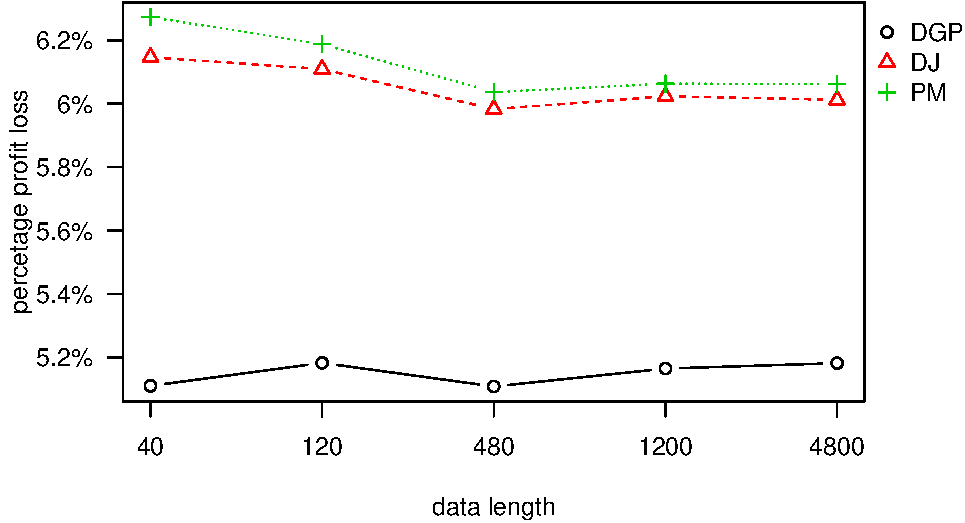
\includegraphics[width=\textwidth]{information-plot_files/figure-latex/AR(1)-1.pdf}
\caption{misleading model AR$(1)$}
\end{subfigure}
\hfill
\begin{subfigure}[b]{0.48\textwidth}
\centering
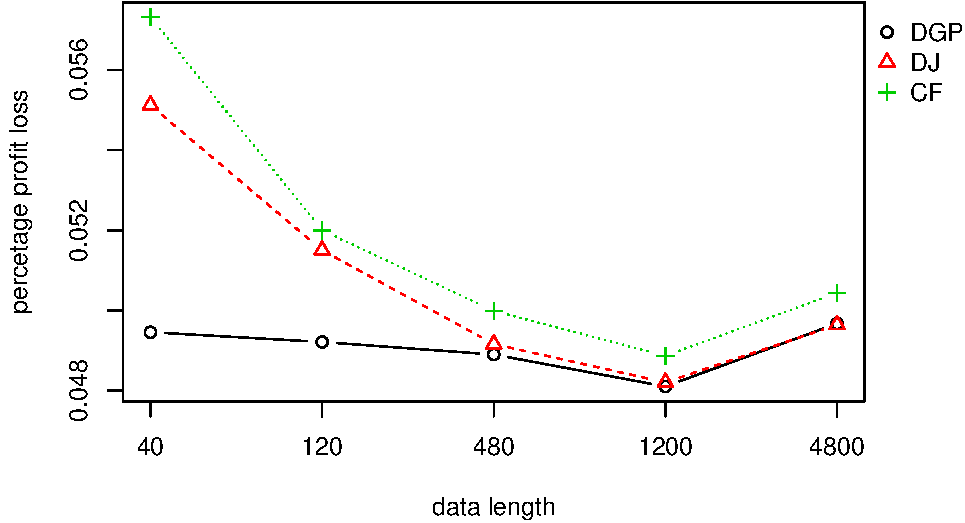
\includegraphics[width=\textwidth]{information-plot_files/figure-latex/SAR(3)(1)_4-1.pdf}
\caption{misleading model ARIMA $(2,0,0)(1,0,0)_4$}
\end{subfigure}
\label{fig:mis}
\end{figure}


\subsection{Nonlinear profit function}
In this subsection, we consider the scenario where the error term of the demand follows normal distribution, and the model of the data generating process is known, but the underlying profit function is nonlinear\footnote{$
        \pi(Q,y)=
        \begin{cases}
            20y-8Q-4(Q-y)+5\E[\min \{(Q-y),u\}],& \text{if } Q\geq y\\
            20Q-8Q-0.01(y-Q)^2,& \text{if } Q< y,
        \end{cases}$ and $u\sim \mathcal{N}(30,5^2)$} (solution see \cite{KK18}).
In this scenario, we explore how the performance changes on both the proposed method and the disjoint method when we alter the profit function to nonlinear. We don't have to make any change to the proposed method, since it makes no assumption to the solution of profit function. However, a simulation algorithm will be used in order to generate the optimal quantile solution of the profit function for the disjoint method. The disjoint method will still be operated in two phases. Mean and variance of the demand will be forecasted in the first phase, and the approximated quantile 0.56 will be used to generate the optimal quantity in the second phase. In the experiment, both the percentage profit loss and the service level will be concerned. The data will still be generated from ARIMA $(1,0,0)(1,0,0)_4$ process, and we use the performance of DGP to compare with both methods. 

The results can be seen in Figure \ref{fig:non}. We can see that the percentage profit loss of the proposed method is very similar to that of the disjoint method in every data size. Regarding to the service level, the proposed method can easily approach the target service level when the data size is small, while the disjoint method needs more data to reach the target service level. Moreover, the proposed method doesn't need any numerical methods or simulation methods to solve for the optimal quantile solution of the profit function. Therefore, it generally requires less computational time.

\begin{figure}[ht]
\centering
\caption{Performance vs. data size with nonlinear profit function}
\begin{subfigure}[b]{0.48\textwidth}
\centering
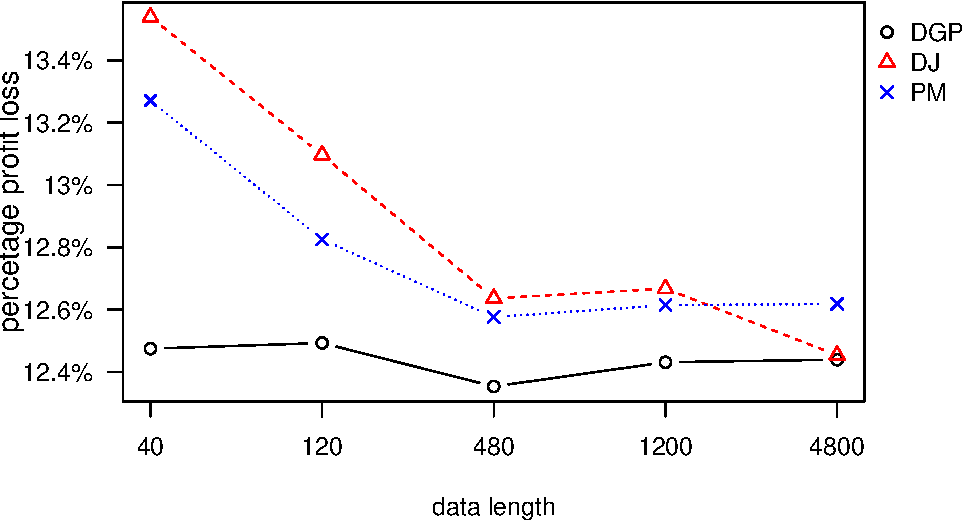
\includegraphics[width=\textwidth]{nonlinear-plot_files/figure-latex/ppl-1.pdf}
\caption{percentage profit loss vs. data size}
\end{subfigure}
\hfill
\begin{subfigure}[b]{0.48\textwidth}
\centering
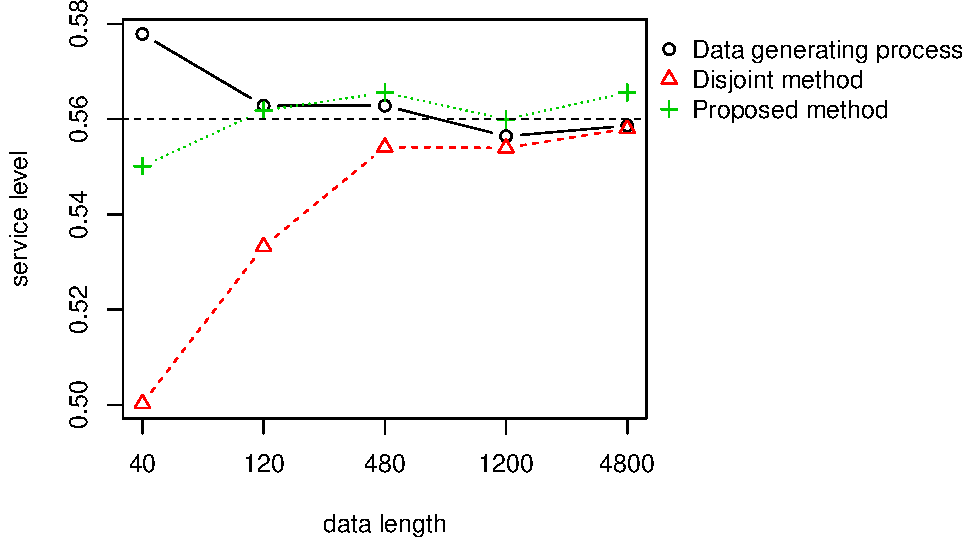
\includegraphics[width=\textwidth]{nonlinear-plot_files/figure-latex/sl-1.pdf}
\caption{service level vs. data size}
\end{subfigure}
\label{fig:non}
\end{figure}


\subsection{Error term misspecification}
In this subsection, we are interested in explore the behavior of our proposed method in the scenario where the error term is misspecified. Particularly, we generate our data from ARIMA $(1,0,0)(1,0,0)_4$ with error term follows Laplace$(0,141)$. Therefore, the mean and variance will be as same as $\mathcal{N}(0,200^2)$. As before, we assume that the model of the data generating process is known, and the underlying profit function is linear where $p=20$, $v=10$, $c_h=-3$, $c_s=-7$. However, we fail to know the true distribution of the error term, and still assume it follows normal distribution $\mathcal{N}(0,200^2)$.


\section{Concluding Remarks} \label{se:end}
This paper presents the framework of a new integrated approach to NVPs. The method is flexible, and doesn't make assumptions about demand distribution nor the solution of profit function. It could generate stable outcomes even in the case we possess misleading information or make wrong assumptions.

We illustrate and compare the proposed method with conventional disjoint method in computational experiments. As expected, the proposed method can achieve as same level of performance as disjoint method in classic NVPs, while provides marvelous results when the scenario become complicated. The results of experiment also backup our proof on the transformation property between proposed method and quantile regression in the linear profit function case. Besides, the proposed method behaves well in the nonlinear profit function case where the quantile regression is no longer functional.

For future research, more scenarios of experiment should be considered and tested. Only a few particular examples are used in our paper. In order to provide more robust conclusion, more examples in each scenario are also requested. Moreover, it is interested to consider using a nonlinear form of regression model to estimate the order quantity.
%%%%%%%%%%%%%%%%%%%%%%%%%%%%%%
\printbibliography

%%%%%%%%%%%%%%%%%%%%%%%%%%%%%%
\newpage
\begin{center}
{\bf\Large Appendices}
\end{center}

\appendix

\section{Scale and Shift Invariance}
\label{app:A}

For invariance with respect to scaling:
\[
    \begin{aligned}
        \hat{\boldsymbol{\beta}}(a\mathbf{y},\mathbf{X})
        &=\text{argmax}_{\boldsymbol{\beta}\in \mathbb{R}^{p+1}}\displaystyle\sum_{t=1}^s{\pi(\mathbf{x}_t^{\mathsf{T}}\boldsymbol{\beta},ay_t)}\\
        &=\text{argmin}_{\boldsymbol{\beta}\in \mathbb{R}^{p+1}}\displaystyle\sum_{t=1}^s{\{c_o[\mathbf{x}_t^{\mathsf{T}}\boldsymbol{\beta}-ay_t]^{+}+c_u[ay_t-\mathbf{x}_t^{\mathsf{T}}\boldsymbol{\beta}]^{+}\}}\\
        &=\text{argmax}_{\boldsymbol{\beta}\in \mathbb{R}^{p+1}}\displaystyle\sum_{t=1}^s{\pi\left(\mathbf{x}_t^{\mathsf{T}}\frac{\boldsymbol{\beta}}{a},y_t\right)}\\
        &=a\hat{\boldsymbol{\beta}}(\mathbf{y},\mathbf{X}).
    \end{aligned}
\]

\noindent
For invariance with respect to shifting:
\[
    \begin{aligned}
        &\hat{\boldsymbol{\beta}}(\mathbf{y}+\mathbf{X}\gamma,\mathbf{X})\\
        &\quad=\text{argmax}_{\boldsymbol{\beta}\in \mathbb{R}^{p+1}}\displaystyle\sum_{t=1}^s{\pi(\mathbf{x}_t^{\mathsf{T}}\boldsymbol{\beta},y_t+\mathbf{x}_t^{\mathsf{T}}\gamma)}\\
        &\quad=\text{argmin}_{\boldsymbol{\beta}\in \mathbb{R}^{p+1}}\displaystyle\sum_{t=1}^s{\{c_o[\mathbf{x}_t^{\mathsf{T}}\boldsymbol{\beta}-y_t-\mathbf{x}_t^{\mathsf{T}}\gamma]^{+}+c_u[y_t+\mathbf{x}_t^{\mathsf{T}}\gamma-\mathbf{x}_t^{\mathsf{T}}\boldsymbol{\beta}]^{+}\}}\\
        &\quad=\text{argmax}_{\boldsymbol{\beta}\in \mathbb{R}^{p+1}}\displaystyle\sum_{t=1}^s{\pi[\mathbf{x}_t^{\mathsf{T}}(\boldsymbol{\beta}-\gamma),y_t]}\\
        &\quad=\hat{\boldsymbol{\beta}}(\mathbf{y},\mathbf{X})+\gamma.
    \end{aligned}
\]

\section{Invariance under Reparameterization}
\label{app:B}

Define
    \[
        \mathbf{D}=\mathbf{X}A
        =\begin{pmatrix}
            \mathbf{d}_1^{\mathsf{T}}\\
            \mathbf{d}_2^{\mathsf{T}}\\
            \vdots\\
            \mathbf{d}_s^{\mathsf{T}}
        \end{pmatrix}
        =\begin{pmatrix}
            \mathbf{x}_{1}^{\mathsf{T}}\mathbf{a}^1&\mathbf{x}_1^{\mathsf{T}}\mathbf{a}^2&\cdots &\mathbf{x}_1^{\mathsf{T}}\mathbf{a}^{p+1}\\
            \mathbf{x}_2^{\mathsf{T}}\mathbf{a}^1&\mathbf{x}_2^{\mathsf{T}}\mathbf{a}^2&\cdots &\mathbf{x}_2^{\mathsf{T}}\mathbf{a}^{p+1}\\
            \vdots &\vdots &\ddots &\vdots \\
            \mathbf{x}_s^{\mathsf{T}}\mathbf{a}^1&\mathbf{x}_s^{\mathsf{T}}\mathbf{a}^2&\cdots &\mathbf{x}_s^{\mathsf{T}}\mathbf{a}^{p+1}
        \end{pmatrix},
    \]
    where $\mathbf{a}^n$ is the $n$th column of matrix $A$. We have
    \[
        \begin{aligned}
            &\hat{\boldsymbol{\beta}}(\mathbf{y},\mathbf{X}A)\\
            &\quad=\text{argmax}_{\boldsymbol{\beta}\in \mathbb{R}^{p+1}}\displaystyle\sum_{t=1}^s{\pi(\mathbf{d}_t^{\mathsf{T}}\boldsymbol{\beta},y_t)}\\
            &\quad=\text{argmin}_{\boldsymbol{\beta}\in \mathbb{R}^{p+1}}\displaystyle\sum_{t=1}^s{\{c_o[\mathbf{d}_t^{\mathsf{T}}\boldsymbol{\beta}-y_t]^{+}+c_u[y_t-\mathbf{d}_t^{\mathsf{T}}\boldsymbol{\beta}]^{+}\}}.
        \end{aligned}
    \]
    Note that
    \[
        \begin{aligned}
            \mathbf{d}_t^{\mathsf{T}}\boldsymbol{\beta}
            &=\displaystyle\sum_{n=1}^{p+1}\mathbf{x}_t^{\mathsf{T}}\mathbf{a}^n\beta_n\\
            &=\displaystyle\sum_{n=1}^{p+1}\displaystyle\sum_{m=1}^{p+1}x_{tm}a_{mn}\beta_n\\
            &=\displaystyle\sum_{m=1}^{p+1}x_{tm}\mathbf{a}_m^{\mathsf{T}}\boldsymbol{\beta}\\
            &=\mathbf{x}_t^{\mathsf{T}}A\boldsymbol{\beta},
        \end{aligned}
    \]
    where $a_{mn}$ is the element at $m$th row and $n$th column of $A$.
    From this, we have:
    \[
        \begin{aligned}
            &\hat{\boldsymbol{\beta}}(\mathbf{y},\mathbf{X}A)\\
            &\quad=\text{argmin}_{\boldsymbol{\beta}\in \mathbb{R}^{p+1}}\displaystyle\sum_{t=1}^s{\left\{c_o\left[\mathbf{x}_t^{\mathsf{T}}A\boldsymbol{\beta}-y_t\right]^{+}+c_u\left[y_t-\mathbf{x}_t^{\mathsf{T}}A\boldsymbol{\beta}\right]^{+}\right\}}\\
            &\quad=\text{argmax}_{\boldsymbol{\beta}\in \mathbb{R}^{p+1}}\displaystyle\sum_{t=1}^s{\pi(\mathbf{x}_t^{\mathsf{T}}A\boldsymbol{\beta},y_t)}\\
            &\quad=A^{-1}\hat{\boldsymbol{\beta}}(\mathbf{y},\mathbf{X}).
        \end{aligned}
    \]
    
\section{Equivalence to Quantile Regression}
\label{app:C}
We are here to show the loss function used in our proposed method is transformable to the typical loss function of quantile regression. In quantile regression, the loss function is defined as \cite{KH01}:
\[
    \hat{\boldsymbol{\beta}}=\text{argmin}_{\boldsymbol{\beta}\in \mathbb{R}^{p+1}}\displaystyle\sum_{t=1}^s\rho_{\tau}(y_t-\mathbf{x}_t^{\mathsf{T}}\boldsymbol{\beta}),
\]
where $\displaystyle \rho_{\tau}(u)=u(\tau-\mathbb{I}_{(u<0)})$, and $\mathbb{I}$ is an indicator function. Thus, all we need to do is to prove:
\[
    \text{max}\displaystyle\sum_{t=1}^s{\pi(\mathbf{x}_t^{\mathsf{T}}\boldsymbol{\beta},y_t)}=\text{min}\displaystyle\sum_{t=1}^s\rho_{\tau}(y_t-\mathbf{x}_t^{\mathsf{T}}\boldsymbol{\beta}).
\]
We have:
\[
    \min[a,b]=a-[a-b]^+,
\]
and
\[
    a-b=[a-b]^+-[b-a]^+.
\]
We can transform:
\[
    \begin{aligned}
        \pi(\mathbf{x}_t^{\mathsf{T}}\boldsymbol{\beta},y_t)
        &=p\min[\mathbf{x}_t^{\mathsf{T}}\boldsymbol{\beta},y_t]-v\mathbf{x}_t^{\mathsf{T}}\boldsymbol{\beta}-c_h[\mathbf{x}_t^{\mathsf{T}}\boldsymbol{\beta}-y_t]^+-c_s[y_t-\mathbf{x}_t^{\mathsf{T}}\boldsymbol{\beta}]^+\\
        &=p\{\mathbf{x}_t^{\mathsf{T}}\boldsymbol{\beta}-[\mathbf{x}_t^{\mathsf{T}}\boldsymbol{\beta}-y_t]^+\}-v\mathbf{x}_t^{\mathsf{T}}\boldsymbol{\beta}-c_h[\mathbf{x}_t^{\mathsf{T}}\boldsymbol{\beta}-y_t]^+-c_s[y_t-\mathbf{x}_t^{\mathsf{T}}\boldsymbol{\beta}]^+\\
        &=(p-v)\mathbf{x}_t^{\mathsf{T}}\boldsymbol{\beta}-(c_h+p)[\mathbf{x}_t^{\mathsf{T}}\boldsymbol{\beta}-y_t]^+-c_s[y_t-\mathbf{x}_t^{\mathsf{T}}\boldsymbol{\beta}]^+.
    \end{aligned}
\]
Therefore, we have (since $y_t$ is fixed):
\[
    \begin{aligned}
        &\text{max}\displaystyle\sum_{t=1}^s{\pi(\mathbf{x}_t^{\mathsf{T}}\boldsymbol{\beta},y_t)}\\
        &\quad=\text{max}\displaystyle\sum_{t=1}^s\{(p-v)\mathbf{x}_t^{\mathsf{T}}\boldsymbol{\beta}-(c_h+p)[\mathbf{x}_t^{\mathsf{T}}\boldsymbol{\beta}-y_t]^+-c_s[y_t-\mathbf{x}_t^{\mathsf{T}}\boldsymbol{\beta}]^+\}\\
        &\quad=\text{max}\displaystyle\sum_{t=1}^s\{(p-v)[\mathbf{x}_t^{\mathsf{T}}\boldsymbol{\beta}-y_t]-(c_h+p)[\mathbf{x}_t^{\mathsf{T}}\boldsymbol{\beta}-y_t]^+-c_s[y_t-\mathbf{x}_t^{\mathsf{T}}\boldsymbol{\beta}]^+\}\\
        &\quad=\text{max}\displaystyle\sum_{t=1}^s\{(p-v)[\mathbf{x}_t^{\mathsf{T}}\boldsymbol{\beta}-y_t]^+-(p-v)[y_t-\mathbf{x}_t^{\mathsf{T}}\boldsymbol{\beta}]^+\\
        &\qquad-(c_h+p)[\mathbf{x}_t^{\mathsf{T}}\boldsymbol{\beta}-y_t]^+-c_s[y_t-\mathbf{x}_t^{\mathsf{T}}\boldsymbol{\beta}]^+\}\\
        &\quad=\text{min}\displaystyle\sum_{t=1}^s\{(v+c_h)[\mathbf{x}_t^{\mathsf{T}}\boldsymbol{\beta}-y_t]^++(p-v+c_s)[y_t-\mathbf{x}_t^{\mathsf{T}}\boldsymbol{\beta}]^+\}\\
        &\quad=\text{min}\displaystyle\sum_{t=1}^s\{c_o[\mathbf{x}_t^{\mathsf{T}}\boldsymbol{\beta}-y_t]^++c_u[y_t-\mathbf{x}_t^{\mathsf{T}}\boldsymbol{\beta}]^+\}.
    \end{aligned}
\]
By setting $\tau=\nicefrac{c_u}{(c_o+c_u)}$, we have:
\[
    \text{max}\displaystyle\sum_{t=1}^s{\pi(\mathbf{x}_t^{\mathsf{T}}\boldsymbol{\beta},y_t)}=\text{min}\displaystyle\sum_{t=1}^s\{(1-\tau)[\mathbf{x}_t^{\mathsf{T}}\boldsymbol{\beta}-y_t]^++\tau[y_t-\mathbf{x}_t^{\mathsf{T}}\boldsymbol{\beta}]^+\}=\text{min}\displaystyle\sum_{t=1}^s\rho_{\tau}(y_t-\mathbf{x}_t^{\mathsf{T}}\boldsymbol{\beta}).
\]
\end{document}